\section{Results}
\label{sec:results}

The results chapter presents results from both the statistical, and LLM approach previously presented in section \ref{sec:method}.

%%%%%%%%%%%%%%%%%%%%
\subsection{Results: statistical approach}
\label{subsec:results-stat-appoach}

Table \ref{tab:res-aggr-stat-approach} presents aggregated results from the statistical approach, both with and without (w/o) stop-word removal. Highlighted values showcase the best performing model in each category in this iteration.

\begin{table}[ht]
\centering
\resizebox{\columnwidth}{!}{%
\begin{tabular}{lcccc}
\toprule
\textbf{Model/Method} & \textbf{Accuracy} & \textbf{Precision} & \textbf{Recall} & \textbf{F1-score} \\
\midrule
Naive Bayes & 0.56 & 0.56	& 0.56 & 0.53 \\
SVM & 0.48 & 0.48 & 0.48 & 0.47 \\
Random Forest & 0.52 & 0.51	& 0.52 & 0.48 \\
Gradient Boosting & 0.59 & 0.59 & 0.59 & 0.58 \\
\midrule
\textit{Naive Bayes} & 0.57 & 0.57 & 0.57 & 0.54 \\
\textit{SVM} & 0.50 & 0.50 & 0.50 & 0.49 \\
\textit{Random Forest} & 0.52 & 0.52 & 0.52 & 0.49 \\
\textit{Gradient Boosting} & \textbf{0.60} & \textbf{0.60} & \textbf{0.60} & \textbf{0.59} \\
\bottomrule
\end{tabular}
}
\caption{Aggregated results from both statistical approaches. Models in \textit{italic} showcase results with stop-words removed.}
\label{tab:res-aggr-stat-approach}
\end{table}


\setlength{\parindent}{1em}
Gradient Boosting here displays the best performance across all metrics, regardless of stop-word removal. The general accuracy of the statistical approaches is around 48 to 60\%, where again the gradient boosting classifier with stop word removal has the overall best accuracy. Further, figure \ref{fig:conf-matrices-stat-wo} and \ref{fig:conf-matrices-stat} showcase confusion matrices for each method in this iteration. This shows that the category \textit{general pathological conditions} is more difficult for all models to correctly classify compared to the other conditions. Again, gradient boosting outperforms in correctly labeling this condition. Further comparing the results, one can see that stop-word removal increases the predictive performance for \textit{general pathological conditions} across all models, where for example the SVM classifier now predicts 137 of 481 correctly compared to 125 of 481 previously. Overall, the SVM classifier seems to benefit the most from stop-word removal.

\begin{figure}[ht]
    \centering
    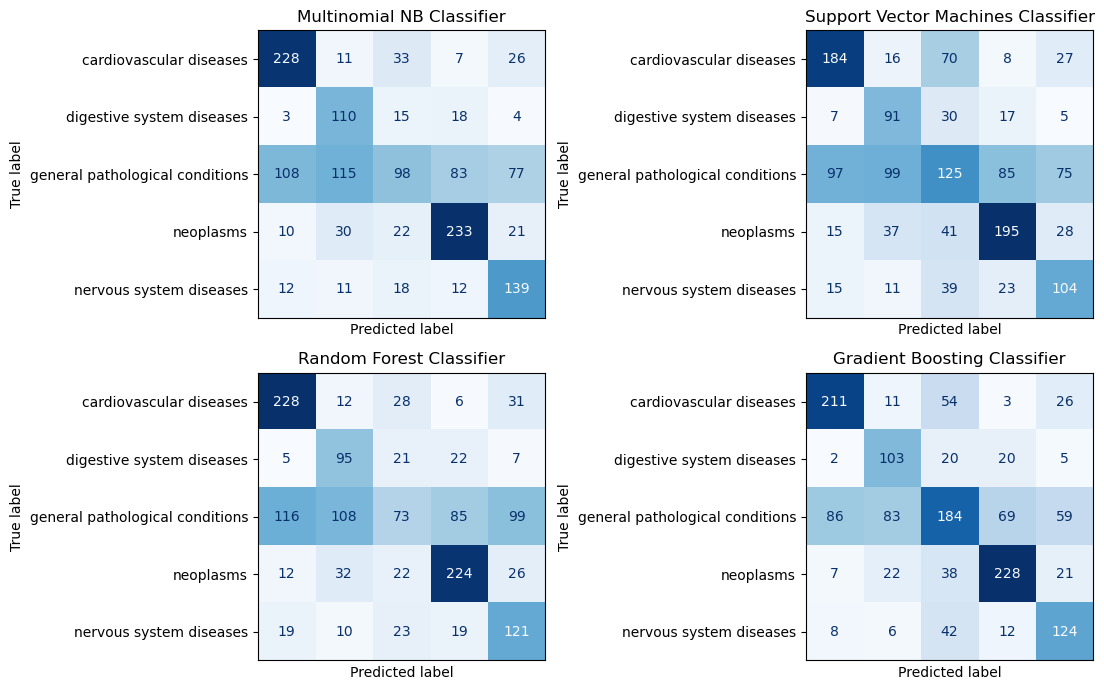
\includegraphics[width=\columnwidth]{report/figures/conf-matrices-stat-wo.png}
    \caption{Confusion matrices for statistical approach w/o stop-word removal.}
    \label{fig:conf-matrices-stat-wo}
\end{figure}
\vspace{-1em}
\begin{figure}[ht]
    \centering
    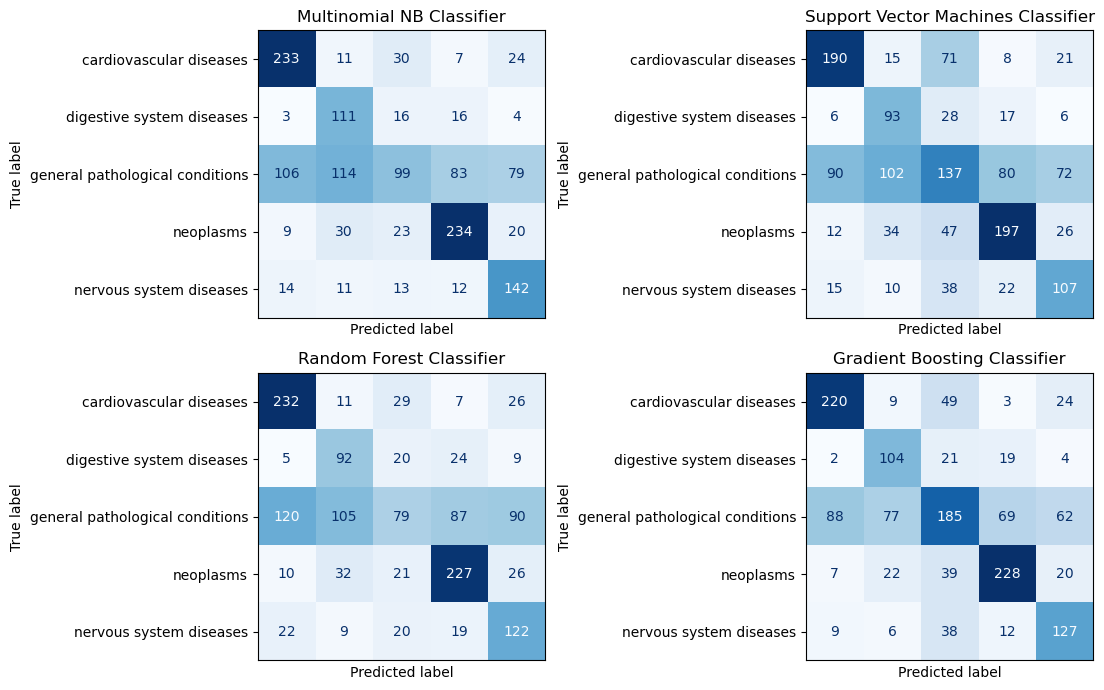
\includegraphics[width=\columnwidth]{report/figures/conf-matrices-stat.png}
    \caption{Confusion matrices for statistical approach with stop-word removal.}
    \label{fig:conf-matrices-stat}
\end{figure}

%%%%%%%%%%%%%%%%%%%%
\subsection{Results: LLM approach}
\label{subsec:results-stat-appoach}

Table \ref{tab:res-aggr-full} presents aggregated results from both the statistical approach, both with and w/o stop-word removal, as well as the LLM approach. Again, highlighted values showcase the best performing model in each category in this iteration.

\begin{table}[ht]
\centering
\resizebox{\columnwidth}{!}{%
\begin{tabular}{lcccc}
\toprule
\textbf{Model/Method} & \textbf{Accuracy} & \textbf{Precision} & \textbf{Recall} & \textbf{F1-score} \\
\midrule
Naive Bayes & 0.56 & 0.56	& 0.56 & 0.53 \\
SVM & 0.48 & 0.48 & 0.48 & 0.47 \\
Random Forest & 0.52 & 0.51	& 0.52 & 0.48 \\
Gradient Boosting & 0.59 & 0.59 & 0.59 & 0.58 \\
\midrule
\textit{Naive Bayes} & 0.57 & 0.57 & 0.57 & 0.54 \\
\textit{SVM} & 0.50 & 0.50 & 0.50 & 0.49 \\
\textit{Random Forest} & 0.52 & 0.52 & 0.52 & 0.49 \\
\textit{Gradient Boosting} & \textbf{0.60} & 0.60 & \textbf{0.60} & \textbf{0.59} \\
\midrule
Zero-shot & 0.55 & 0.59 & 0.55 & 0.52 \\
One-shot & 0.59 & 0.60 & 0.59 & \textbf{0.59} \\
Few-shot & \textbf{0.60} & \textbf{0.61} & \textbf{0.60} & \textbf{0.59} \\
Similarity based & 0.47 & 0.46 & 0.47 & 0.45 \\
\bottomrule
\end{tabular}
}
\caption{Aggregated results from both the statistical and LLM approach. Models in \textit{italic} showcase results with stop-words removed.}
\label{tab:res-aggr-full}
\end{table}

%\setlength{\parindent}{1em}
Here, one can see that the Few-shot prompted GPT-3.5 Turbo model from the LLM approach performs the best out of all tested models, however very similar to gradient boosting in all metrics but one. The One-shot model also displays equally good performance in terms of F1-score. Figure \ref{fig:conf-matrices-llm} displays additional information to the results from the LLM approach in the form of confusion matrices for each tested method. Similar to the statistical approach, \textit{general pathological conditions} seems to be the most difficult to correctly classify, especially for the zero-shot prompted model and the similarity classifier. However, significant improvement can be seen in correctly classifying this condition in the one- and few-shot prompted classifiers. At the same time, a slight decrease in performance compared to the zero-shot prompted model can be seen, for example in the categories digestive system diseases and neoplasms.

\begin{figure}[ht]
    \centering
    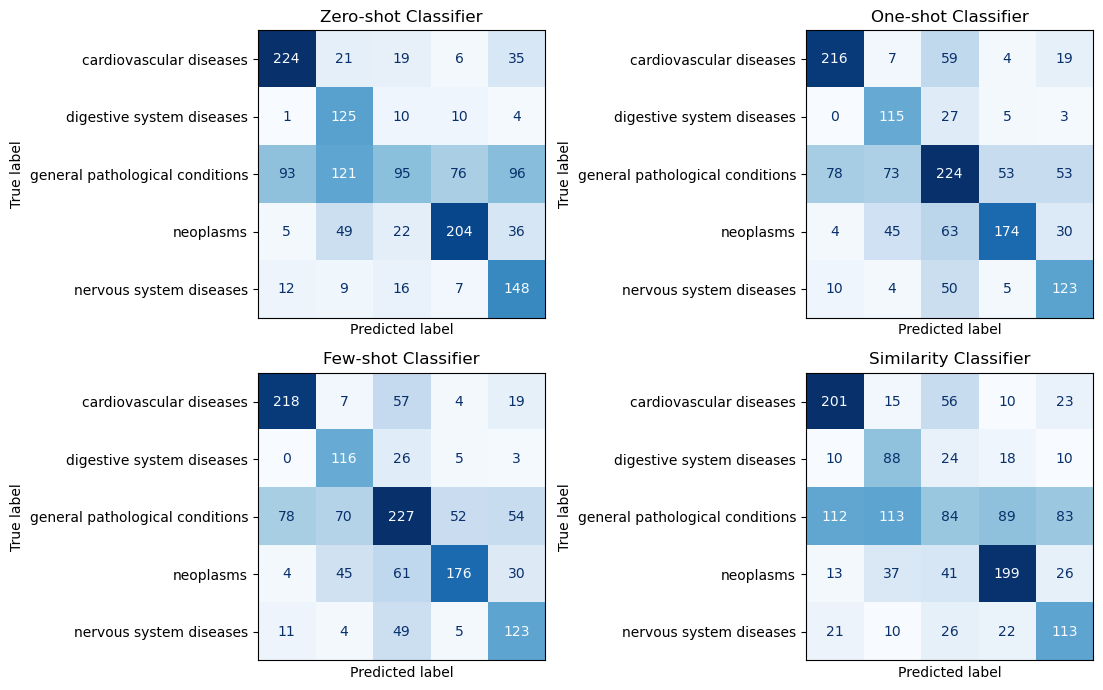
\includegraphics[width=\columnwidth]{report/figures/conf-matrices-llm.png}
    \caption{Confusion matrices for llm approach.}
    \label{fig:conf-matrices-llm}
\end{figure}